% LaTeX dokumentu guztiak zein dokumentu mota den adieraziz hasi behar dira
\documentclass[es]{ifirak}

% ERABILIKO DIREN PAKETEAK %

% listings paketea kodea formateatzeko erabiltzen da
\usepackage{listings}
% Paquete para los acentos
\usepackage[utf8]{inputenc}

% Paketea konfiguratu behar dugu C lengoaiarekin erabiltzeko:
\definecolor{darkgreen}{rgb}{0,0.5,0}
\definecolor{lightgray}{rgb}{0.95,0.95,0.95}
\definecolor{gray}{rgb}{0.65,0.65,0.65}
\lstset{language=C,
		basicstyle=\scriptsize\ttfamily,
		keywordstyle=\color{darkgreen}\bfseries,
		identifierstyle=\color{blue},
		commentstyle=\color{gray}, 
		stringstyle=\ttfamily,
		showstringspaces=false,
		tabsize=2,
		backgroundcolor=\color{lightgray}}


\begin{document}
% Hainbat datu ...
\ikasturtea{2014 - 2015}
\irakasgaia{Minería de Datos}
% Titulua
\title{Cuadernillo de prácticas}
% Zuen izena
\author{Mikel Dalmau}

\maketitle

% Abstract ingurunea hasierako laburpena idazteko erabili
\begin{abstract}
El siguiente documento está compuesto por una serie de prácticas realizadas en la asignatura de Minería de Datos. Estas varían desde la sintesis de artículos de aplicaciones reales de la minería de datos hasta definiciones de terminos relacionados con este ámbito, aunque principalmente se centran en el estudio de clasificadores utilizando como herramienta el software Weka.
\end{abstract}

% Testua egituratzeko section, subsection, subsubsection, subsubsection eta paragraph komandoak dituzue
\section{Introducción, lecturas de aplicaciones reales de la minería de datos }
\paragraph{}
 El objetivo de esta practica es ilustrar sobre las aplicaciones de la minería de datos y ver la horizontalidad de la disciplina, esto es, su posible aplicación en casi cualquier ámbito.
\subsection{Mining for cheap flights}

\begin{enumerate}

\item  Con esta aplicación se pretende anticipar a los cambios de precios de los vuelos para aconsejar a los usuarios sobre cuando comprar o no los billetes de avión. La variable clase a predecir será si un vuelo va a cambiar de precio y cuando.

\item Creo que hay más que suficientes casos como para crear un modelo de clasificación robusto. Siempre que un precio cambie y sea posible asociar dicho cambio a algunos de los factores ambientales más influyentes, el modelo aprenderá.

\item Tal y como se indica en el artículo variables como los cambios estacionales, festivales, convenciones, o actos en general que pudieran movilizar a una cantidad grande de personas, tendrán sin duda efecto en los precios, también es probable que causas climáticas como huracanes o nubes de ceniza puedan influir. 

Creo que estas variables por sí solas no tienen suficiente fuerza como para predecir efectivamente las fluctuaciones de los precios.

\item Creo que es necesaria la minería de datos en este entorno por varias razones, entre ellas, la ingente cantidad de vuelos y cambios constantes en los precios, la enorme cantidad de factores ambientales que pueden afectar a dichos precios y las complejas relaciones que estos factores externos pueden crear. 

Creo que ningún experto sería capaz de anticiparse a los precios de los vuelos y 	cualquier modelo predictivo no basado en el aprendizaje automático terminaría por 	quedarse obsoleto.


\item Me ha llamado la atención el hecho de que todavía sea necesaria la asistencia del ojo humano para descubrir patrones que los ordenadores todavía no son capaces. 

Esto tiene mucho sentido para mi, la supervivencia del hombre siempre ha estado unida a su capacidad para identificar patrones y reconocer pautas comunes, al fin y al cabo una máquina no va a ser capaz de superar en unos pocos años lo que la evolución ha hecho durante miles.

\end{enumerate}





\subsection{Aprendizaje automático para interpretar el ADN}
\begin{enumerate}

\item  En este artículo explican como se busca mejorar en el diagnostico y prevención de enfermedades. La variable clase sería una enfermedad específica en una población específica.

\item  En el caso del genoma, los casos mas interesantes serían aquellos de 	las personas afectadas por la enfermedad o aquellos genomas que muestren resistencia a la misma. Creo que conseguir casos suficientes será un tarea larga y harán falta años para crear modelos robustos.

\item  Resultados clínicos, población, secuencias genómicas iguales o similares. Creo que pueden ser variables muy significativas a la hora de predecir la variable clase.

\item  En el entorno del ADN, aunque la mejora ha sido enorme, secuenciar el 	genoma completo supone un gran coste, esto nos da una idea de la cantidad de datos que existe y que para analizarlos es necesaria la minería de datos. 

Aunque haya médicos que pudieran dar sentido a estos datos, no sería posible para ellos ni para ningún humano hacerlo al nivel que ofrece la minería de datos.

\item  No conozco aplicaciones parecidas, y pienso que esta traerá grandes mejoras a la medicina. Me ha llamado la atención el gasto de tiempo y dinero que supone secuenciar el genoma completo, espero que con los años estos costos se abaraten todavía más.   

\end{enumerate}


\section{ Clasificador del vecino más próximo K-NN }



\subsection{Parámetros del clasificador "IBk": "KNN", "distanceWeighting"} 

\paragraph{}
KNN(K-Nearest Neighbours): K es el número de vecinos más cercanos que se utilizarán para predecir la clase del objeto. La clase del objeto a predecir será la más común entre el número de vecinos seleccionados. Si $K = 1$, asignaremos al objeto la clase del vecino más cercano.
Aparte de la clasificación, también podemos utilizar el método de KNN para la regresión, esto es, inferir un valor nominal o continuo a partir de sus vecinos.
\paragraph{}
DistanceWeighting: Tanto para la clasificación como para la regresión puede ser útil asignar pesos a los vecinos según su proximidad, es lógico pensar que los vecinos más próximos al objeto a clasificar influyen más que los lejanos.
\paragraph{}
Existen distintos modos de valorar la distancia, en Weka podemos encontrar $Weight$ by $1/distance$, donde el peso del vecino a la hora de calcular la media será inversamente proporcional su distancia respecto del objeto a clasificar. La métrica de la distancia en este caso debe estar definida por una función de disimilitud como por ejemplo la distancia Euclídea o la distancia de Minkowski.
\paragraph{}
Para el otro caso, donde $Weight=1 – distance$ en cambio, la métrica estará definida por una función de similitud, donde el rango de valores que puede tomar la distancia está contenido en el intervalo $[0, 1]$. La similitud o cercanía entre los datos será mínima en 0 y máxima en 1 (Son el mismo punto). El coseno y la correlación de Pearson son medidas de similitud.

\subsection{Pruebas del clasificador}
\paragraph{}
La próxima tabla  y gráficas muestran los resultados obtenidos en las pruebas de Weka, para el clasificado KNN con distintas métricas y la técnica de validación Hold Out, utilizando dos tercios de los datos para crear el modelo y un tercio para el testeo.

\begin{table}[htbp]
\centering
\begin{tabular}{c|c|c|c}
K & Sin Peso &$ Peso = 1/d$ & $Peso = 1-d$\\
\hline
1 & 67.1233 & 67.1233 & 67.1233\\
3 & 63.0137 & 61.6438 & 61.6438\\
5 & 61.6438 & 63.0137 & 61.6438\\
7 & 57.5342 & 60.274 & 58.9041\\
9 & 56.1644 & 60.274 & 58.9041\\
11 & 57.5342 & 61.6438 & 57.5342\\
\end{tabular}
\caption{Resultados K-NN con Weka}\label{table}
\end{table}

\begin{figure}[htbp]
\centering
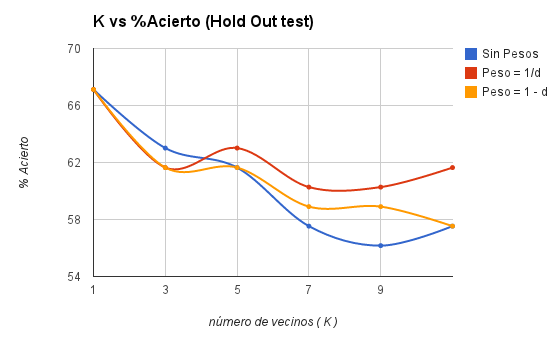
\includegraphics[width=0.8\textwidth]{1kvsAciertos.png}
\caption{Representación gráfica de la Tabla 1}\label{figure}
\end{figure}

\paragraph{}
Lo mas destacable de los resultados, es que la mejor tasa de acierto se logra para $K  = 1$, donde la distancia es irrelevante, a partir de ahí, la tasa de acierto baja bastante en los tres métodos. 
\paragraph{}
Aunque para 3 vecinos, el método Sin Pesos consigue una mejor tasa que los otros dos, podemos apreciar que según aumentamos el número de vecinos las distancias empiezan influir más en la clasificación que la clase más común. 
\paragraph{}
Finalmente la imagen muestra que independientemente del método y del número de vecinos que escojamos las tasas de acierto son bajas y no mejoran, esto probablemente será por la técnica de validación, se consiguen mejores tasas de acierto utilizando la técnica de validación cruzada que trabaja mejor en conjuntos de datos pequeños.

\subsection{Clasificadores Lazy} 
\paragraph{}
El aprendizaje vago, a diferencia del entusiasta, donde el sistema intenta generalizar los datos de entrenamiento antes de recibir preguntas, como podría ser un árbol de clasificación, lo que hace es eperar a recibir la pregunta para realizar la generalización. 
\paragraph{}
Por ejemplo, una de las ventajas del clasificador KNN frente a un árbol, es que la función objetivo será aproximada localmente (vecinos más próximos), si surgiera algún cambio en el dominio el árbol no sería capaz de clasificarlo y el KNN si.

\section{Términos de la minería de datos en inglés }

\begin{itemize}

\item \emph{Accuracy}: Este termino no tiene traducción en español, pero lo podemos definir como la relación entre la Precisión y la Exactitud. Refiriéndose la Precisión a la dispersión entre los datos medidos y el real, una medida de precisión muy común es la desviación estándar, y la Exactitud, a cuan cerca está el dato medido del real, cuanto más pequeño sea el error, mayor será la exactitud. 

\item \emph{Attribute-feature}: Cuando la clasificación de los datos y la base de datos se hace y está compuesta por atributos que describen propiedades del mundo real.

\item \emph{Categorical variable}: Llamamos categóricas a las variables que no pueden ser cuantificadas, como por ejemplo los colores. 

\item \emph{Continuous variable}: Estas son las variables que sí pueden ser medidas, como la altura o el peso de una persona.

\item \emph{Classifier}: Es un algoritmo que se encarga de la clasificación, esto es, decide a que  categoría o clase pertenece una observación, el algoritmo se desarrolla sobre un conjunto de entrenamiento en el que ya conocemos la categoría de cada observación.

\item \emph{Confusion matrix}: Es una matriz cuadrada que enfrenta las clases reales de un conjunto de datos frente a las clases predichas por un clasificador para ese mismo conjunto. Sirve para visualizar la bondad de dicho clasificador de una forma desglosada. 

\item \emph{True positive rate}: Muestra el porcentaje de bien clasificados entre los que han sido clasificados como parte de una clase.

\item \emph{False positive rate}: Muestra el porcentaje de mal clasificados entre los que no han sido clasificados como parte de una clase.

\item \emph{Cross-validation}: Es un método de validación iterativo, que divide el conjunto de datos en una serie de bloques, realizará entonces tantas iteraciones como bloques de datos haya, utilizando en cada una un bloque como conjunto de testeo y el resto como conjunto de aprendizaje. 

\item \emph{Data cleaning}: Es el proceso en el que se tratan los datos recogidos para su posterior análisis, por ejemplo, eliminando las tuplas con campos vacíos o perdidos(missing values) o eliminando los datos que no se ajustan al comportamiento general(outliers).

\item \emph{Data mining}: Es el proceso de análisis de las grandes bases de datos y descubrir patrones utilizando técnicas de inteligencia artificial, aprendizaje automático, estadística y sistemas de bases de datos.

\item \emph{Instance}: Llamamos instancia a cada tupla de la base de datos u observación individual, que está compuesta por una serie de atributos y una o varias clases.

\item \emph{Knowledge discovery}: LLamamos knowledge discovery al proceso de extraer información útil de una colección de datos.

\item \emph{Machine learning}: Es una rama de la ciencia de computadores y de la estadística, consiste en que las máquinas puedan aprender de los datos que reciben en vez de tener unas instrucciones específicas.

\item \emph{Missing value}: Cuando a alguna observación o tupla de la base de datos le falta el valor de algún atributo.

\item \emph{Model}: Un modelo es una función que en base a los atributos de una observación le asignara una clase determinada. 

\item \emph{Supervised learning}: Consiste en inducir un modelo a partir de un conjunto de entrenamiento en el que conocemos la clase de los datos, al contrario que en el no supervisado, donde no tenemos clase y hay que tratar de buscar patrones y también se carece de métodos para evaluar el error o las posibles soluciones.

\end{itemize}

\section{Estimación del porcentaje de bien clasificados}

\paragraph{}
El problema de esta práctica trata de predecir si un paciente muestra síntomas de tener diabetes o no, para ello se utilizan variables como la presión sanguínea, concentración de glucosa, masa corporal y edad, entre otras. La variable clase a predecir es binaria, siendo 1 para cuando el test ha sido positivo, esto es, el paciente probablemente tenga diabetes, y 0 en el caso contrario. 

\subsection{Resultados de las pruebas en Weka} 
\paragraph{}
Los valores y porcentajes hacen referencia al número de bien clasificados.


\begin{table}[htbp]
\centering
\begin{tabular}{c|c|c}
Alg & número & \% \\
\hline
3-NN & 659 &  85.8073 \\
J48 & 646 & 84.1146 \\
\end{tabular}
\caption{Método no honesto}\label{table}
\end{table}

\begin{table}[htbp]
\centering
\begin{tabular}{c|c|c}
Alg & número & \% \\
\hline
3-NN & 195 &  74.7126 \\
J48 & 199 & 76.2452 \\
\end{tabular}
\caption{Método H (66\% train - 33\% test)}\label{table}
\end{table}

\begin{table}[htbp]
\centering
\begin{tabular}{c|c|c}
Alg & número & \% \\
\hline
3-NN & 278 &  72.3958 \\
J48 & 285 & 74.2188 \\
\end{tabular}
\caption{Método H (50\% train - 50\% test)}\label{table}
\end{table}

\begin{table}[htbp]
\centering
\begin{tabular}{c|c|c}
Alg & número & \% \\
\hline
3-NN & 553 &  72.0052 \\
J48 & 581 & 75.6510 \\
\end{tabular}
\caption{10-fold cross-validation}\label{table}
\end{table}

\begin{table}[htbp]
\centering
\begin{tabular}{c|c|c}
Alg & número & \% \\
\hline
3-NN & 548 &  71.3542 \\
J48 & 556 & 72.3958 \\
\end{tabular}
\caption{5-fold cross-validation}\label{table}
\end{table}

\begin{table}[htbp]
\centering
\begin{tabular}{c|c|c}
Alg & número & \% \\
\hline
3-NN & 569 &  74.0885 \\
J48 & 567 & 73.8281 \\
\end{tabular}
\caption{Leave-one-out }\label{table}
\end{table}

\begin{table}[htbp]
\centering
\begin{tabular}{c|c|c|c|c|c|c}
3-NN&&&&&& Media \\
\hline
número & 190 		  & 195 		 & 195 		 & 192 		 & 193 		 & 193 		   \\
 \%    & 72.7969       & 74.7126 & 74.7126 & 73.5632 &73.9464 &73.9436\\
 &&&&&&\\
J48&&&&&&\\
\hline
 número & 188 		  & 185 		 & 200 		 & 195 		 & 181 		 & 190		   \\
 \%    & 72.0307       & 70.8812 & 76.6284 & 74.7126 &69.3487 &72,7202\\
\end{tabular}
\caption{Submuestreo aleatorio (66\% train - 33\% test) }\label{table}
\end{table}

\begin{figure}[htbp]
\centering
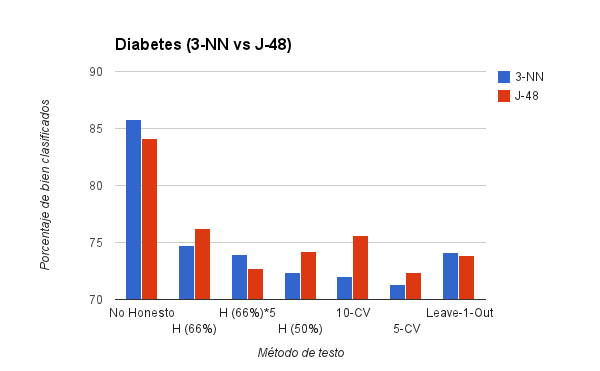
\includegraphics[width=0.8\textwidth]{2diabetes.png}
\caption{Representación gráfica de los datos expuestos en las Tablas 2-8}\label{figure}
\end{figure}


\subsection{Interpretación de los resultados}
\paragraph{}
En un primer vistazo al gráfico anterior vemos que destaca el porcentaje de bien clasificados obtenido por la técnica de validación No Honesto, un resultado totalmente esperado dada la naturaleza de esta técnica, que hace las pruebas con el mismo conjunto que utiliza para crear el modelo. La gran diferencia entre este resultado y los obtenidos para las otras técnicas, que utilizan el mismo algoritmo de aprendizaje nos da una idea de la poca fiabilidad de dicho porcentaje.
\paragraph{}
Respecto a los próximos resultados, los obtenidos por el método Hold-out(66\%) y el submuestreo aleatorio, cabe destacar la gran varianza y la baja media obtenida por el algoritmo C4.5 frente a lo obtenido por el algoritmo 3-NN donde los resultado apenas varían. Podríamos pensar que los algoritmos Lazy como K-NN son más estables frente a cambios en el conjunto de entrenamiento que los entusiastas como el árbol de clasificación C4.5, o podría deberse a que en este caso la distribución de la variable clase no está balanceada, hay mas clases de un caso que de otro. 
\paragraph{}
En cualquier caso los resultados anteriores nos invitan a que no nos fiemos de los siguientes, los obtenidos por la técnica Hold-out (50\%).
\paragraph{}
Siguiendo el histograma vemos los resultados obtenidos por la técnica 10-fold cross-validation y 5-fold cross-validation, que no tienen especial interés mas que comentar otra vez la diferencia entre los resultados del algoritmo C4.5.
\paragraph{}
En esta técnica se construyen N+1 modelos, donde N es el número de pliegues, las primeras N veces, Weka utilizara una fracción de los datos (N-1)/N para formar el conjunto de entrenamiento, 90\% en nuestro caso, y finalmente utilizará todo el conjunto para crear el último modelo.
\paragraph{}
Por último vemos los resultados de la técnica Leave-1-Out, que son casi idénticos para los dos algoritmos que hemos probado y son sin duda los más fiables de todos. 
La técnica Leave-1-Out es exactamente igual que cross-validation pero se realizaran tantas iteraciones como datos haya en el conjunto, tomando en cada una de estas un único dato como conjunto de testeo y el resto como entrenamiento. En nuestro caso se trata de 768-folds cross-validation y desde luego ha sido la más exigente computacionalmente para Weka, y este es el mayor inconveniente de esta técnica, el bajo grado de error se paga a nivel computacional y esto posiblemente la haga inviable en muchas situaciones.
\paragraph{}
El mensaje que se puede leer durante la ejecución de la validación cruzada es Building model for fold 'X', y es tal y como he explicado arriba, Weka creando los distintos modelos para cada iteración.

\section{Árboles de clasificación }

\paragraph{}
En este problema, se trata de predecir la cantidad de trébol blanco que crecerá o la persistencia de este en un verano tórrido en una de las tres zonas de estudio en el año 1994, basándose en las medidas para ese año y los dos anteriores de otras legumbres, hierbas, plantas y del trébol blanco en sí.
\paragraph{}
La variable clase a predecir es un valor continuo por lo que se ha discretizado en cuatro intervalos distintos:

\begin{displaymath}
   0\leq WhiteClover-94<8.8225 	
\end{displaymath}
\begin{displaymath}
  8.8225\leq WhiteClover-94<17.645  	
\end{displaymath}
\begin{displaymath}
 17.645\leq WhiteClover-94<26.4675 
\end{displaymath}
\begin{displaymath}
26.4675\leq WhiteClover-94\leq 35.29 
\end{displaymath}

\paragraph{}
Los árboles producidos por el método C4.5 con y sin poda son idénticos en todas sus hojas y variables intermedias excepto por un sub-árbol que surge de la variable $cocksfoot-93 \rightarrow > 12.5$, en este caso, el criterio de poda determina que desarrollar la rama amplifica el error cometido o no lo disminuye. 

\paragraph{}
Si el árbol podado tiene 9 variables intermedias o nodos y 10 hojas, y el sub-árbol que desarrollamos tiene 2 nodos y 9 hojas, el árbol resultante de no aplicar el proceso de poda es la suma de los dos anteriores pero sin contar la hoja que sería nodo, entonces tiene 11 variables intermedias y 18 hojas.
\paragraph{}
Como podemos ver no todas las variables originales aparecen en los árboles, esto se debe a que el método de construcción de árboles clasifica comenzando por la variable más informativa y se desarrolla hasta clasificar correctamente el conjunto de entrenamiento o hasta que el error sea irreducible (con poda), en la mayoría de casos no son necesarias mas que unas pocas variables para la clasificación correcta.
\paragraph{}
Sobre los números que se distinguen entre paréntesis en cada hoja, el de la izquierda puede representar el número de objetos del conjunto de entrenamiento que se clasifican de esa manera, esto es, que sus variables han ido cumpliendo las condiciones que les ha arrastrado desde la raíz hasta dicha hoja. Los de la derecha podrían representar el número de mal clasificados en dicha hoja.\\

\vspace{0.4cm}
Árbol podado,10-fold cross-validation\\

$$TPR = 0.619		$$	
$$FPR = 0.322$$

Árbol podado, Hold-Out (66\%)\\

$$TPR =0.476    			$$
$$FPR = 0.398$$

\paragraph{}
True Positive Rate y False Positive Rate, indican el ratio de bien clasificados y mal clasificados respectivamente, aunque pueden desglosarse y verse sólo para una determinada variable, tal y como se puede ver en la matriz de confusión.
\paragraph{}
Vemos que los ratios son distintos para los distintos métodos, esto es normal ya que en ambos utilizamos distintos conjuntos de entrenamiento y distintos conjuntos de testeo.

\section{Clasificadores Bayesianos, naive Bayes}
\paragraph{}
En esta practica vamos a trabajar sobre la base de datos Hepatitis y con el clasificador naive bayes pero en vez de utilizar todas las variables nos vamos a limitar a cuatro, Fatiga, Malestar, Anorexia e Higado grande.

\vspace{0.5cm}
\textbf{Estadísticos del clasificador}

\paragraph{}
Class\\
Die(D) 	\hspace{2.5cm}	$P (D) = 0.21$\\
Live(L)		\hspace{2.5cm}  $P (L) = 0.79$\\
\paragraph{}
Fatigue (F)\\
$P(F | D ) = 0.91$ \hspace{2.5cm}	$P(\overline{F} | D ) = 0.9$\\
$P(F | L ) = 0.57$ \hspace{2.5cm}	$P(\overline{F} | L ) = 0.43$\\
\paragraph{}
Malaise (M)\\
$P( M | D ) = 0.71$ \hspace{2.5cm}	$P(\overline{M} | D ) = 0. 29$\\
$P( M | L) = 0.31$ \hspace{2.5cm}	$P(\overline{M} | L ) = 0.69$\\
\paragraph{}
Anorexia (A)\\
$P(A  | D) = 0.32$ \hspace{2.5cm}	$P(\overline{A} | D ) = 0.68$\\
$P(A | L ) = 0.19$ \hspace{2.5cm}	$P(\overline{A} | L ) = 0.81$\\
\paragraph{}
Liver Big (LB)\\
$P(LB | D) = 0.86$	\hspace{2.5cm}  $P(\overline{LB} | D ) = 0.14$\\
$P(LB | L) = 0.81$  \hspace{2.5cm}  $P(\overline{LB} | L) = 0.19$\\

\textbf{Clasificar un nuevo caso dada la siguiente evidencia:}\\
$$ Fatigue = yes;\hspace{0.2cm} Malaise = yes;\hspace{0.2cm} Anorexia = no;\hspace{0.2cm} Liver\hspace{0.05cm} big = yes;$$
Calculamos las probabilidades conjuntas de la clase y los distintos hallazgos:\\
\begin{displaymath}
 P (C = D | ( F , M ,\overline{A} , LB) )\hspace{0.1cm}  \alpha \hspace{0.1cm}  p(D)\hspace{0.1cm} \Pi \hspace{0.1cm}p( Xi | C = D) =
\end{displaymath}
\begin{displaymath}
= p(D)\times P(F | D )\times P( M | D )\times P(\overline{A}  | D ) \times P(LB | D) = 0.21 \times 0.91 \times 0.71 \times 0.68 \times 0.97 = 0.077
\end{displaymath}

\begin{displaymath}
P (C = L | ( F , M ,\overline{A} , LB) ) \hspace{0.1cm} \alpha \hspace{0.1cm} p(L)\hspace{0.1cm} \Pi \hspace{0.1cm}p( Xi | C = L)  =
\end{displaymath}
\begin{displaymath}
= p(L)\times P(F | L )\times P( M | L )\times P(\overline{A}  | L ) \times P(LB | L) = 0.79 \times 0.57 \times 0.31 \times 0.81 \times 0.81 = 0.092
\end{displaymath}
Finalmente si dividimos cada resultado por la suma de los dos obtenemos la probabilidad condicionada:\\
Probabilidad de que el nuevo caso sea de la clase Die.\\
\begin{displaymath}
 P(C = D | ( F , M , \overline{A} , LB) ) = 0.46 \rightarrow 46\% 
\end{displaymath}\\
Probabilidad de que el nuevo caso sea de la clase Live.\\

\begin{displaymath}
 P(C = L | ( F , M , \overline{A} , LB) ) = 0.54 \rightarrow 54\%
\end{displaymath}\\
El clasificador apostará por el segundo caso, donde la clase es LIVE.\\

\textbf{Clasificar un nuevo caso dada la siguiente evidencia:}\\

$$Fatigue = no;\hspace{0.2cm} Malaise = no;\hspace{0.2cm} Anorexia = no;\hspace{0.2cm} Liver\hspace{0.05cm} big = no$$
Calculamos las probabilidades conjuntas de la clase y los distintos hallazgos:\\
\begin{displaymath}
P (C = D | ( \overline{F} , \overline{M} , \overline{A} , \overline{LB}) ) \hspace{0.1cm} \alpha  \hspace{0.1cm} p(D) \hspace{0.1cm} \Pi \hspace{0.1cm}p( Xi | C = D)=
\end{displaymath}
\begin{displaymath}
= p(D)\times P(\overline{F} | D )\times P( \overline{M} | D )\times P(\overline{A}  | D ) \times P(\overline{LB} | D) = 0.21 \times 0.9  \times 0.29 \times 0.68 \times 0.14 =0.0052179
\end{displaymath}

\begin{displaymath}
P (C = L | ( \overline{F} , \overline{M} ,\overline{A} , \overline{LB}) )\hspace{0.1cm}  \alpha  \hspace{0.1cm}p(L)\hspace{0.1cm} \Pi \hspace{0.1cm} p( Xi | C = L)  =
\end{displaymath}
\begin{displaymath}
=p(L)\times P(\overline{F} | L )\times P( \overline{M} | L )\times P(\overline{A}  | L ) \times P(\overline{LB} | L) = 0.79 \times 0.43 \times 0.69 \times 0.81 \times 0.19 = 0.036073
\end{displaymath}
Probabilidad de que el nuevo caso sea de la clase Die.\\
\begin{displaymath}
 P(C = D | ( \overline{F} , \overline{M} , \overline{A} , \overline{LB}) ) = 0.13 \rightarrow 13\%
\end{displaymath}\\
Probabilidad de que el nuevo caso sea de la clase LIVE.\\
\begin{displaymath}
 P (C = L | ( \overline{F} , \overline{M} , \overline{A} , \overline{LB}) ) =  0.97 \rightarrow 97\%
\end{displaymath}\\
El clasificador apostará por el segundo caso, donde la clase es LIVE.\\

\paragraph{}
En mi opinión las probabilidades $p(Xi=xi|C=die)$ y $p(Xi=xi|C=live)$ para una variable $X_i$ deberían ser diferentes par ayudarnos a diferenciar entre las distintas clases, esto es que su entropía sea baja, como LiverBig por ejemplo, sin embargo Fatiga que tiene probabilidades condicionadas muy parecidas y una entropía muy alta, lo que no nos ayuda tanto a clasificar.

\section{Preprocesamiento de datos, Discretización de variables ordinales-numéricas}

\textbf{Parámetro bins y makeBinary}
\paragraph{}
La función del parámetros bins es indicar el número de particiones que deseamos para nuestra variable discreta, nótese que para bins 1 la variable no aporta ninguna información ya que siempre toma el mismo valor y para bins 2 la variable sería binaria. 
\paragraph{}
Otra forma de lograr este efecto es indicar como true el campo makeBinary, en este caso es necesario que bins sea 2, en caso contrario lo que sucederá es que Weka copiará las variables de forma que cada una de las copias de la original será binaria pero tendrá intervalos distintos, si las agrupáramos obtendríamos la variable original con los intervalos para dicho parámetro bins.\\

\textbf{UseEqualFrequency}
\paragraph{}
La función del parámetro utilizar misma frecuencia es indicar que a la hora de  crear las particiones queremos que estas se hagan de forma cada una de estas contenga el mismo número de datos.
Equal Width
\paragraph{}
Cuando discretizamos por igual anchura, tomamos la diferencia máxima entre los datos, el máximo menos el mínimo y la dividimos por el número bins deseado. De esta forma todos los intervalos tendrán la misma anchura, excluyendo claro los intervalos laterales.
\paragraph{}
La principal diferencia entre los dos métodos anteriores de cara a la clasificación es que en el primer caso la entropía de la variable siempre será máxima, habrá siempre el mismo número de valores para cada caso, mientras que en el segundo método esto no sucedería, muchos valores pueden agruparse en un solo intervalo.\\

\textbf{Cambios en el pseudohistograma}
\paragraph{}
El efecto que se aprecia en el histograma es la reducción de columnas, inicialmente Weka ya discretiza los valores en unos intervalos con el fin de representarlos en el pseudohistograma, aunque las variables sigan siendo numéricas. El número de columnas que surgen es precisamente el que hayamos indicado en el parámetro bins.\\

\textbf{Tipos de valores toman las variables discretizadas}
\paragraph{}
Una vez discretizadas, las variables toman valores que representan intervalos, esto es, representan los infinitos números contenidos entre los extremos del intervalo pudiendo representar o no los extremos, el intervalo que contiene a los extremos es abierto y si no los contiene si es cerrado, también llamamos cerrados a los intervalos que contiene un extremo abierto y otro cerrado. 
\paragraph{}
A pesar de esta distinción no todos los intervalos tienen las mismas propiedades, algunos de ellos tienen una longitud de intervalo y estos son los que llamamos finitos, mientras los que tienen como extremo -inf o +inf no tienen longitud. Como se puede observar en Weka siempre nos encontraremos con intervalos de este tipo, ya que son necesarios para cubrir toda la recta de los números reales.
Efecto de la discretización sobre variables nominales
\paragraph{}
El efecto sobre estas variables ha sido nulo, la variable clase se mantiene igual antes y después de discretizar. Esto es porque sería imposible discretizar algo que ya es discreto como los colores, aunque si los valores estuvieran representados por intervalos si que podrían unirse entre ellos y reducir el número de valores posibles, aún así Weka ignora cualquier variable de tipo nominal.
Efecto de la discretización en la clasificación

\begin{figure}[htbp]
\centering
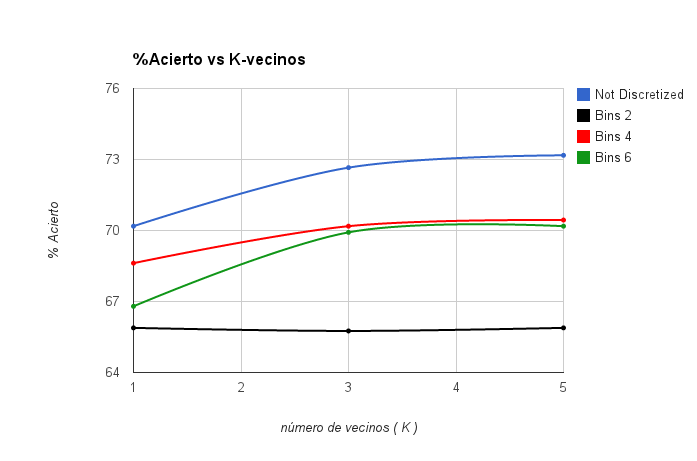
\includegraphics[width=0.8\textwidth]{image.png}
\caption{Representación gráfica de los datos tomados en Weka para distintos valores de Bins}\label{figure}
\end{figure}

\paragraph{}
En cierto modo los resultados eran de esperar, hay muchas variables y al fin y al cabo tampoco interesa tanto o no es necesario para clasificar conocer el valor exacto de cada una, es suficiente con saber mas o menos por que rangos se mueven.


\section{Preprocesamiento de datos}

\subsection{Utilizando el filtro RemoveWithValues}
\paragraph{}
\textbf{Parámetros}

\begin{itemize}
\item \emph{AttributeIndices:} Especifica el rango de atributos en los que aplicar el filtro.
\item \emph{InvertSelection:} Invierte la selección realizada.
\item \emph{NominalIndices:} Rango de valores para la selección de atributos nominales. Firs y Last son valores válidos, a los atributos nominales les son asignados unos índices para identificarlos.
\item \emph{SplitPoint:} Valor númerico que sirve para la selección de atributos numéricos, se seleccionaran aquellos inferiores al indicado.
\end{itemize}

\textbf{Proceso de filtrado}

\paragraph{}
\begin{figure}[htbp]
\centering
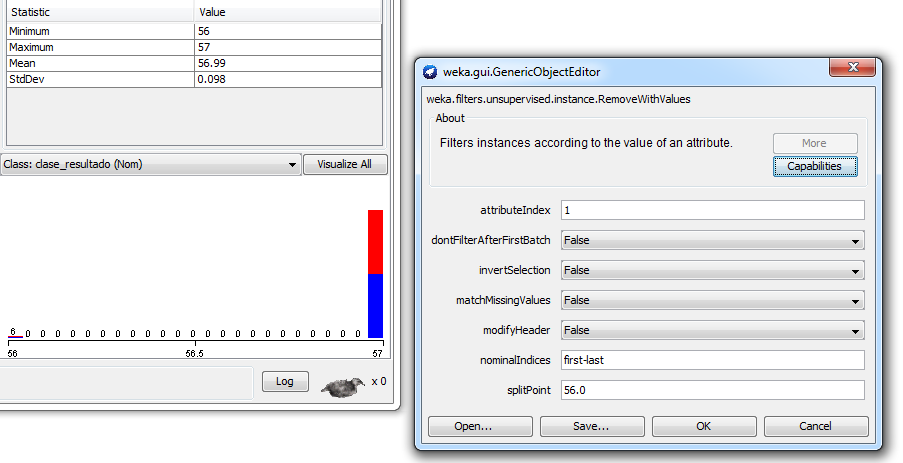
\includegraphics[width=0.8\textwidth]{PrimerFiltro.png}
\caption{Captura de las opciones del filro RemoveWithValues para el primer filtrado.}\label{figure}
\end{figure}

En este primer paso he seleccionado la variable de índice uno que indica el código de temporada, puesto que la deseada, 2012-2013 es la última temporada es suficiente con indicar su código en split-point y todos las demás serán eliminadas por el filtro.

\begin{figure}[htbp]
\centering
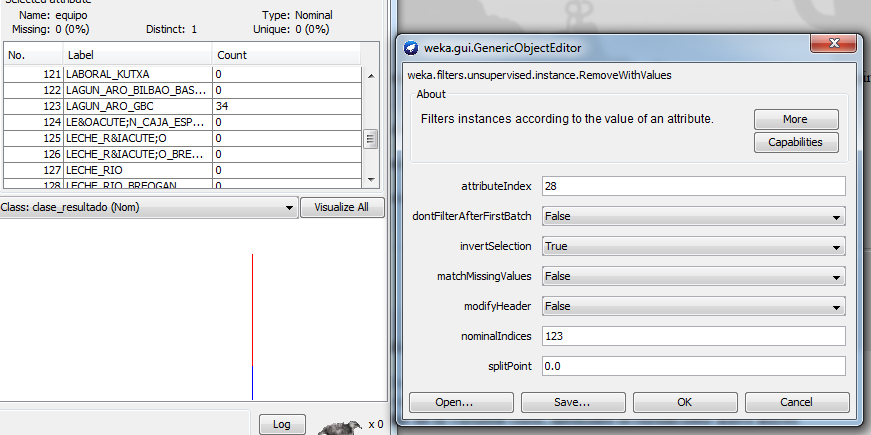
\includegraphics[width=0.8\textwidth]{SegundoFiltro.png}
\caption{Captura de las opciones del filro RemoveWithValues para el segundo filtrado.}\label{figure}
\end{figure}

\paragraph{}
En este segundo paso he seleccionado la variable de índice 28 que indica el equipo, luego como sólo me interesaba un equipo, LAGUN\_{ARO}\_{GBC}, he indicado su índice en la variable nominal índices y he invertido la selección para que se seleccionen todas aquellas distintas a esta y sean eliminadas por el filtro.
Finalmente la base de datos termina con 34 instancias, el número de partidos jugados por el equipo elegido durante una temporada.

\subsection{Atribute selección}
\paragraph{}
El siguiente es un filtro que selecciona atributos en base un evaluador que valora cuan efectivo es  el atributo a la hora de clasificar, hay numerosas opciones pero yo voy a limitarme a explicar la GainRatioAttributeEval, y un método de búsqueda como Best First Shearch o búsqueda exhaustiva pero en mi caso solo es posible utilizar el método Ranked que evalúa los atributos individualmente.
\paragraph{}
Respecto a GainRatioAttributeEval, evalua el ratio de ganancia de un atributo con respecto a la clase y en base a este ratio valora el atributo. La siguiente formula es la que se utiliza para hallar los ratios de ganancia, vemos como se hace la diferencia entre las entropías de la clase y la de la clase condicionada al atributo, de esta forma si la entropía condicionada disminuye  el valor será positivo.
$$GainR(Class, Attribute) = (H(Class) - H(Class | Attribute)) / H(Attribute).$$
\paragraph{}
Respecto a Ranked, este dispone de una serie de opciones que sirven para limitar el número de atributos a analizar o índicar límites en estos.

\begin{figure}[htbp]
\centering
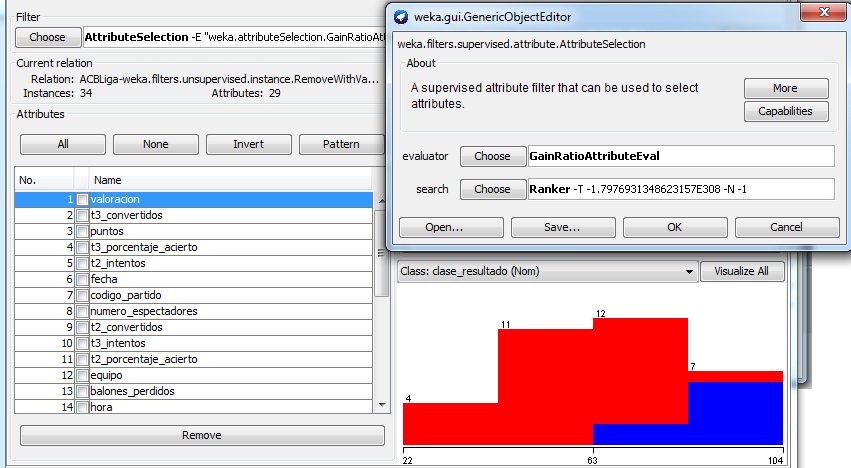
\includegraphics[width=0.8\textwidth]{AtributeSelect.png}
\caption{Captura de las opciones del filtro AtributeSelect}\label{figure}
\end{figure}

\paragraph{}
En la imagen anterior se puede apreciar una re-ordenación de los atributos según el ratio de ganancia.

\subsection{Remove Percentage}
\paragraph{}
Este filtro es muy sencillo y su única función es eliminar un porcentaje de los datos que se indica en la opción percentage, su utilización puede ser interesante en bases de datos grandes. La opción invertSelection, sólo invierte el porcentaje de datos a seleccionar, no tiene mayor relevancia.

\begin{figure}[htbp]
\centering
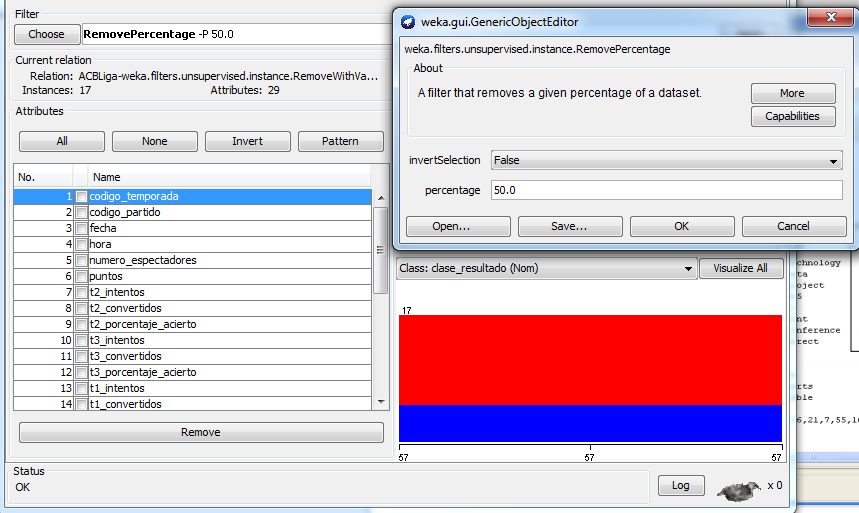
\includegraphics[width=0.8\textwidth]{Removepercentage.png}
\caption{Representación gráfica de los datos tomados en Weka para distintos valores de Bins}\label{figure}
\end{figure}

\paragraph{}
Puede observarse en la imagen que el número de instancias se ha reducido a la mitad.

\section{Clasificadores Bayesianos: aumentados a árbol (TAN-'tree') y k-dependiente ('k-db')}
\paragraph{}
En esta tarea vamos a trabajar con redes bayesianas, pero esta vez ya no se tratará del bayes ingenuo, donde las variables eran condicionalmente independientes dada la clase, esta vez en cambio serán dependientes de un número máximo k de variables.
\paragraph{}
Tras ejecutar en Weka el clasificador bayesiano k2 con 2 padres o arcos máximos a cada variable, sobre la base de datos Hepatitis.arff

\begin{figure}[htbp]
\centering
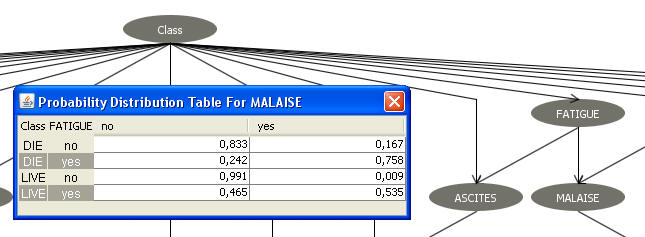
\includegraphics[width=0.8\textwidth]{3Malestar.png}
\caption{Ventana de estadísticos del nodo malestar en Weka}\label{figure}
\end{figure}

\paragraph{}
En la imagen anterior se aprecia una tabla muestra la distribución de probabilidades condicionadas para la variable Malestar. A la izquierda de la tabla se ven la clase y la Fatiga como variables condicionadoras, la clase siempre condicionará a la variable, se ha seleccionado la Fatiga porque es la variable que comparte la mayor información mutua con Malestar.

$$p (Malaise=no \hspace{0.1cm}|\hspace{0.1cm} Class=die , Fatigue=yes) = 0,242$$
$$p (Malaise=yes \hspace{0.1cm}|\hspace{0.1cm}Class=die , Fatigue=yes) = 0,758$$
$$p (Malaise=no \hspace{0.1cm}|\hspace{0.1cm} Class=die , Fatigue=no) = 0,833$$
$$p (Malaise=yes \hspace{0.1cm}|\hspace{0.1cm} Class=die , Fatigue=no) = 0,167$$
$$p (Malaise=no \hspace{0.1cm}|\hspace{0.1cm} Class= live , Fatigue=yes) = 0,465$$
$$p (Malaise=yes \hspace{0.1cm}|\hspace{0.1cm} Class= live , Fatigue=yes) = 0,535$$
$$p (Malaise=no \hspace{0.1cm}|\hspace{0.1cm} Class= live , Fatigue=no) = 0,991$$
$$p (Malaise=yes \hspace{0.1cm}|\hspace{0.1cm} Class= live , Fatigue=no) = 0,009$$
\paragraph{}
Decimos que las probabilidades anteriores son condicionadas porque el valor de la  Fatiga o la Clase afectan a la probabilidad de que haya malestar o no. Por ejemplo, una variable cualquiera, edad, si la edad no influye en el malestar entonces no lo condiciona, si influye entonces si lo condiciona.
\paragraph{}
Dada una evidencia fijada, la suma de las probabilidades a posteriori es uno ya que es la suma de todos los casos posibles y la probabilidad de que suceda alguno  de esos casos es total, la demostración es trivial . 
\paragraph{}
Tal y como he indicado con colores en las probabilidades de arriba observamos que cuando no hay fatiga (azul), las probabilidades de que haya malestar son muy bajas, esto es, la entropía de la distribución es muy baja y la clasificación es mucho más clara, en este caso la variable condicionadora es muy influyente, sin embargo, cuando si hay fatiga (naranja) la entropía es muy alta y por lo tanto, la información que nos aporta es menor.
\paragraph{}
\textbf{LIVER\_{BIG} y  LIVER\_{FIRM}}

\begin{figure}[htbp]
\centering
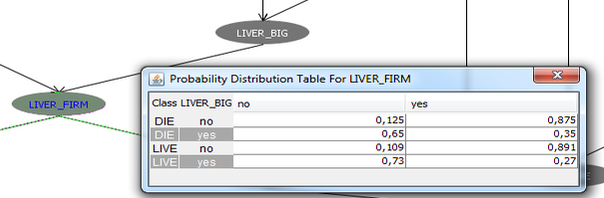
\includegraphics[width=0.8\textwidth]{4LiverFirm.png}
\caption{Ventana de estadísticos del nodo Hígado Firme en Weka}\label{figure}
\end{figure}

\paragraph{}
En la anterior imagen podemos apreciar que cuando el hígado no es grande las probabilidades de que sea firme son muy altas y esto es lo que hace tan influyente a la variable LIVER\_{BIG} a la hora de clasificar LIVER\_{FIRM}, mientras que cuando el hígado sí es grande, la distribución tiene mayor entropía y por lo tanto se nos hace más difícil determinar si tendrá el hígado firme o no, esto es, nos aporta menos información.
\paragraph{}
Tras ejecutar en Weka el clasificador bayesiano k2 con 3 padres o arcos máximos a cada variable, sobre la base de datos Hepatitis.arff, procedemos a analizar la variable bilirubina y su distribución de probabilidades.
\paragraph{}
La variable bilirubina tiene tres padres que la condicionan, por lo tanto tendrá tantas distribuciones de probabilidades como evidencias distintas puedan formarse, dado que todas las variables son binarias, sólo pueden tomar dos casos distintos, el número de evidencias posibles será .
\paragraph{}
Los valores de probabilidad reflejados en la tabla de bilirubina son los siguientes:

$$p (Bilirubin= (-\infty, 1.65] \hspace{0.1cm} |\hspace{0.1cm} Class=die , Anorexia=no, Varices=no) = 0.656$$
$$p (Bilirubin= (1.65, \infty,)  \hspace{0.1cm}|\hspace{0.1cm} Class=die , Anorexia=no, Varices=no) = 0.344$$
$$p (Bilirubin= (-\infty,, 1.65]  \hspace{0.1cm}| \hspace{0.1cm}Class=die , Anorexia=no, Varices=yes) = 0.312$$
$$p (Bilirubin= (1.65, \infty,)  \hspace{0.1cm}|\hspace{0.1cm} Class=die , Anorexia=no, Varices=yes )= 0.688$$

$$p (Bilirubin= (-\infty,, 1.65] \hspace{0.1cm} |\hspace{0.1cm} Class=die , Anorexia=yes, Varices=no) = 0.214$$
$$p (Bilirubin= (1.65, \infty,) \hspace{0.1cm} |\hspace{0.1cm} Class=die , Anorexia=yes, Varices=no) = 0.786$$
$$p (Bilirubin= (-\infty,, 1.65] \hspace{0.1cm}|\hspace{0.1cm} Class=die , Anorexia=yes, Varices=yes) = 0.3$$
$$p (Bilirubin= (1.65, \infty,)  \hspace{0.1cm}|\hspace{0.1cm} Class=die , Anorexia=yes, Varices=yes) = 0.7$$

$$p (Bilirubin= (-\infty,, 1.65]  \hspace{0.1cm}|\hspace{0.1cm} Class=live , Anorexia=no, Varices=no) = 0.923$$
$$p (Bilirubin= (1.65, \infty,)  \hspace{0.1cm}|\hspace{0.1cm} Class=live , Anorexia=no, Varices=no) = 0.077$$
$$p (Bilirubin= (-\infty,, 1.65] \hspace{0.1cm} |\hspace{0.1cm} Class=live , Anorexia=no, Varices=yes) = 0.9$$
$$p (Bilirubin= (1.65, \infty,)  \hspace{0.1cm}|\hspace{0.1cm} Class=live , Anorexia=no, Varices=yes) = 0.1$$

$$p (Bilirubin= (-\infty,, 1.65] \hspace{0.1cm} | \hspace{0.1cm}Class=live , Anorexia=yes, Varices=no) = 0.775$$
$$p (Bilirubin= (1.65, \infty,)  \hspace{0.1cm}|\hspace{0.1cm} Class=live , Anorexia=yes, Varices=no) = 0.225$$
$$p (Bilirubin= (-\infty,, 1.65] \hspace{0.1cm} |\hspace{0.1cm} Class=live , Anorexia=yes, Varices=yes) = 0.125$$
$$p (Bilirubin= (1.65, \infty,)  \hspace{0.1cm}|\hspace{0.1cm} Class=live , Anorexia=yes, Varices=yes) = 	0.875$$



%Bibliografia
\begin{thebibliography}{arauak}


\bibitem[D.Garcia]{key-1}Diego Garcia Morate, \emph{Manual de Weka}, Consulta de uso de parámetros en filtros.

\bibitem[Wiki]{key-2} Wikipedia, \emph{Cross validation},\emph{Naive Bayes} , Referencia general para conceptos teóricos y definiciones.

\bibitem[Weka]{key-3} Weka \emph{http://www.cs.waikato.ac.nz/ml/weka/}, página oficial donde descargar el software utilizado.


\bibitem[Pract]{key-4} \emph{http://www.sc.ehu.es/ccwbayes/docencia/md/pages1415/practicas1415.html} Enunciados de las prácticas y acceso a las bases de datos .arff utilizadas.

\end{thebibliography}
\end{document}
